\newpage
\datos{color}{}{}
\section{[4 puntos] Ejercicio 4}
%\addcontentsline{toc}{section}{Ejercicio 1}
\textbf{Estimación del PIB de países.} \\

\textbf{Usa el conjunto de datos del fichero countries.csv disponible en el campus virtual.}\\

\textbf{En este caso, se solicita desarrollar una tarea de regresión donde cada elemento del
conjunto de datos es un país descrito por una serie de características sociales,
económicas, geográficas y demográficas. La variable a predecir es el PIB del país
(\textit{GDP} en inglés de \textit{Gross Domestic Product}).}

\begin{itemize}
    \item \textbf{Preparación de los datos:}
    \begin{itemize}
        \item Antes de empezar elimina la variable “Region” del conjunto de datos, ya
que no la usaremos para predecir.
        \item Además, utiliza la función \texttt{dropna} que elimina de un \textit{dataframe}
        todas las
filas (es decir, observaciones) que tienen un valor perdido (\texttt{na} quiere
decir \textit{not available}) para alguna variable. De esta forma, no tendrás que
preocuparte por imputar un valor a dichas observaciones. \\
Asegúrate de que el \textit{dataframe} resultante no tiene la variable ``Region'', ni
valores perdidos.
    \end{itemize}

    \item \textbf{Considera si debes normalizar o estandarizar las variables antes para usar un
perceptrón multicapa de decisión. Razona tu elección.}

    \item \textbf{Configura una validación cruzada con k=5 y dos perceptrones multicapa:}
    \begin{itemize}
        \item MLP1 con una capa oculta de 200 neuronas
        \item MLP2 con dos capas ocultas de 50 neuronas cada una
    \end{itemize}

    \item \textbf{Puedes usar un valor alpha=0,1.}
    \item \textbf{Asegúrate de que no salen \textit{warnings} indicando que no se ha alcanzado la
convergencia durante el entrenamiento (basta con poner un número de
max\_iter suficientemente grande, p.ej. 3000).}
    \item \textbf{¿Alguno de los dos perceptrones domina al otro? ¿Por qué crees que se
producen las diferencias?} \\
\end{itemize}

A continuación se presenta el \textit{notebook} de \textit{Python} con el que se ha resuelto el ejercicio.
Las justificaciones, respuestas e interpretaciones se incluyen sobre el propio \textit{notebook}.
\addcontentsline{lol}{lstlisting}{4. \; \; \;\textit{Notebook} del ejercicio 4.}
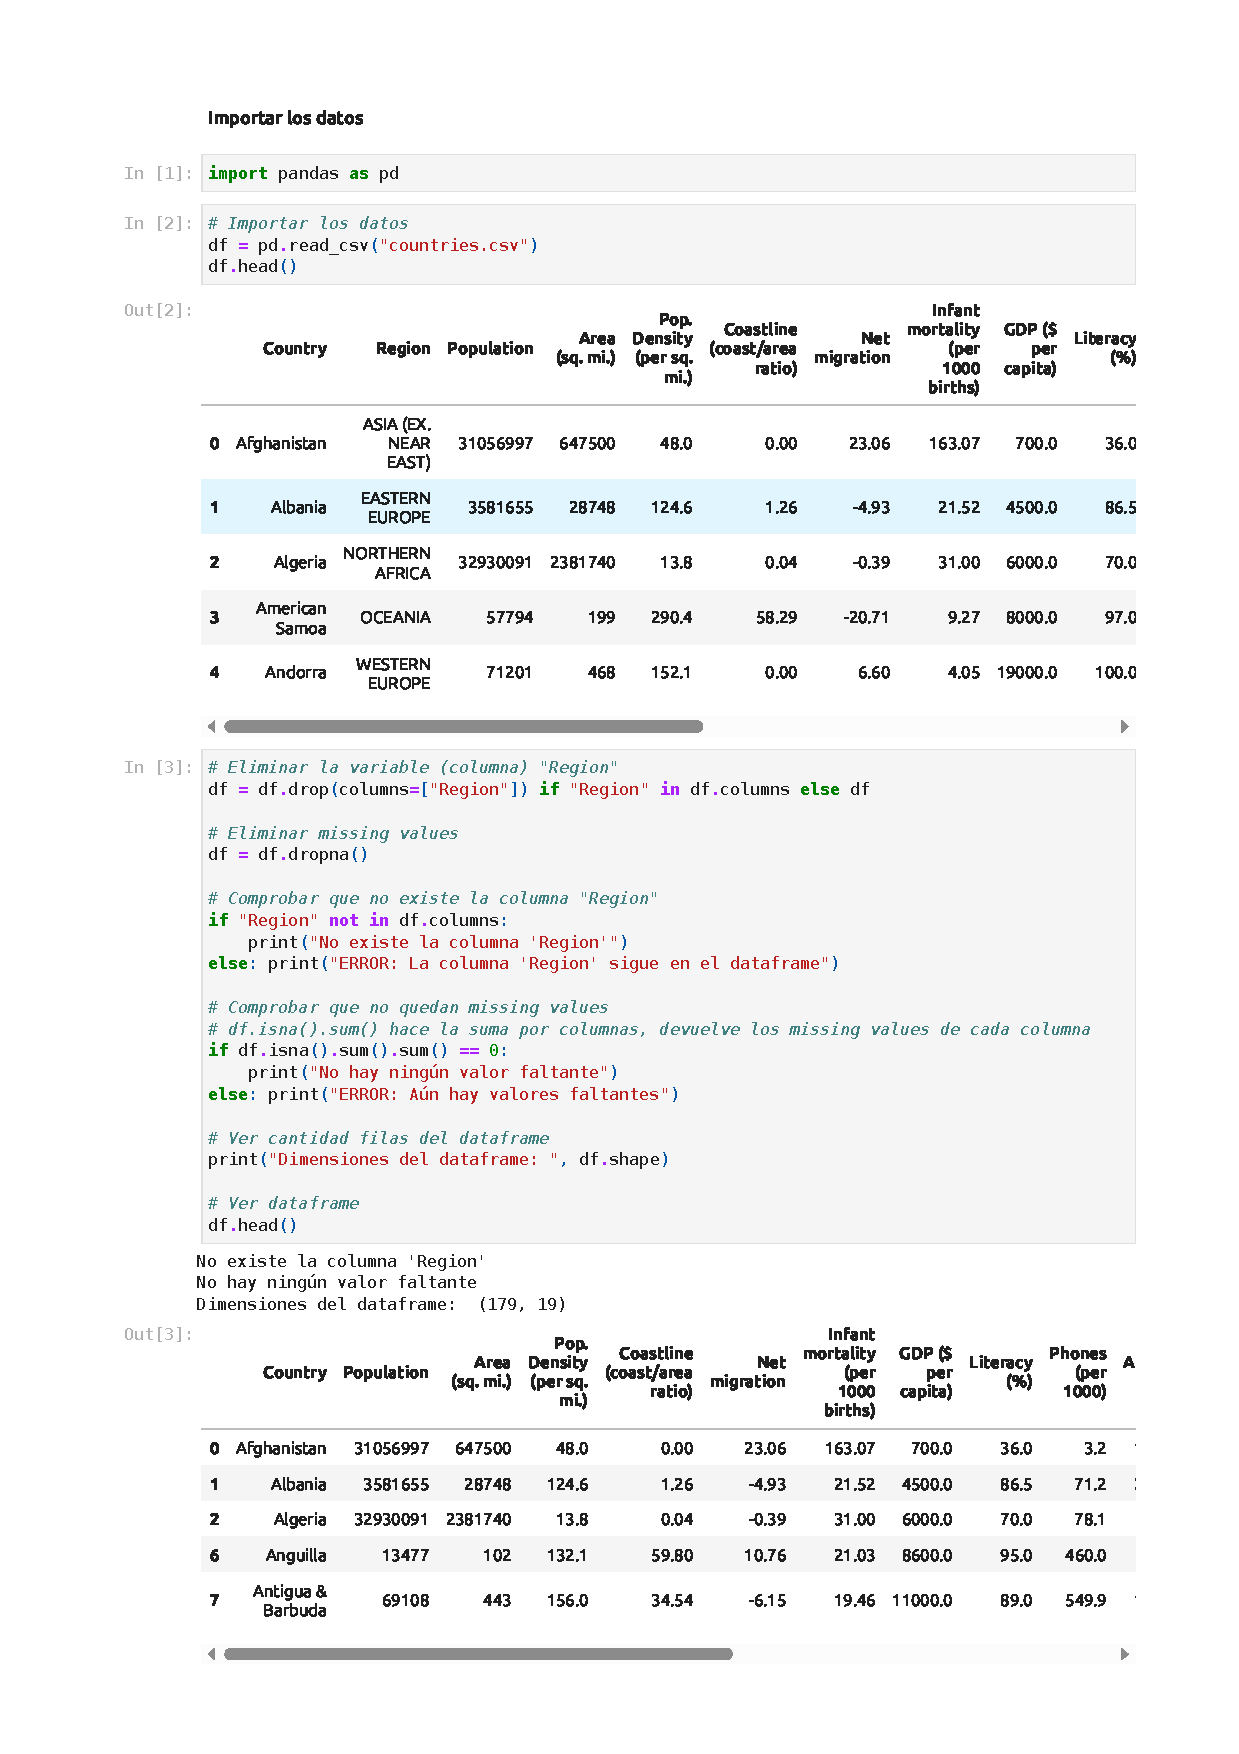
\includepdf[pages=-,pagecommand={\thispagestyle{plain}}]{Code/ejer4_2.pdf}
